\documentclass[10pt,UTF8]{ctexart}


\usepackage[margin=2cm,a4paper]{geometry}
%\usepackage[left=0.75in,top=0.6in,right=0.75in,bottom=1.0in,a4paper]{geometry}

\setmainfont{Caladea}
%% 也可以選用其它字庫:
% \setCJKmainfont[%
%   ItalicFont=AR PL KaitiM GB,
%   BoldFont=Noto Sans CJK SC,
% ]{Noto Serif CJK SC}
% \setCJKsansfont{Noto Sans CJK SC}
% \renewcommand{\kaishu}{\CJKfontspec{AR PL KaitiM GB}}

% 繁體中文
\setCJKmainfont[Path=fonts/ ]{NotoSansTC-Medium.otf}

\usepackage{minted}
\usepackage[breaklinks]{hyperref}

% Picture
% 導言區的此三行無變化
\usepackage{graphicx}
\usepackage{float} 
\usepackage{subfigure}
% 以下是新增的自定義格式更改
\usepackage[]{caption2} %新增調用的宏包
\renewcommand{\figurename}{Fig.} %重定義編號前綴詞
\renewcommand{\captionlabeldelim}{.~} %重定義分隔符
 %\roman 是羅馬數字編號,\alph是默認的字母編號,\arabic是阿拉伯數字編號,可按需替換下一行的相應位置
\renewcommand{\thesubfigure}{(\roman{subfigure})}%此外,還可設置圖編號顯示格式,加括號或者不加括號
\makeatletter \renewcommand{\@thesubfigure}{\thesubfigure \space}%子圖編號與名稱的間隔設置
\renewcommand{\p@subfigure}{} \makeatother

% Math
\usepackage {mathtools}
\usepackage{amssymb}

% Code
\usepackage{listings}
\usepackage{xcolor}
\lstset{
    % backgroundcolor=\color{red!50!green!50!blue!50},
    % 程式碼塊背景色為淺灰色
    rulesepcolor= \color{gray}, % 程式碼塊邊框顏色
    breaklines=true,  % 程式碼過長則換行
    numbers=left, % 行號在左側顯示
    numberstyle= \small,% 行號字型
    % eywordstyle= \color{red,% 關鍵字顏色
    commentstyle=\color{gray}, % 註釋顏色
    frame=shadowbox % 用方框框住程式碼塊
    }

\usepackage{hyperref}

\title{計算機視覺作業}
\author{干皓丞,2101212850, 信息工程學院}

\begin{document}
\maketitle


\section{作業目標與作業狀況}

作業可以從 GitHub 下的 kancheng/kan-cs-report-in-2021 專案找到,作業程式碼與文件目錄為 kan-cs-report-in-2021/CV/cv-final。實際執行的環境與實驗設備為 Google 的 Colab 、MacBook Pro (Retina, 15-inch, Mid 2014) 、 Acer Aspire R7 與 HP Victus (Nvidia GeForce RTX 3060)。

對之前的論文清單做延伸,內容包括但不限於:論文內容、程式碼復現、實驗創新等,形成一份報告。

再對過往 8 篇論文逐一復現的狀況,而第 8 篇的 "Binary TTC: A Temporal Geofence for Autonomous Navigation" 復現相對穩定,但是由於原本研究者的環境是 Linux ,將原本執行的 Linux Shell 的 *.sh 檔案改寫成 PowerShell 的 *.ps1 的寫法,讓成果可以穩定執行。

\begin{figure}[H]
\centering 
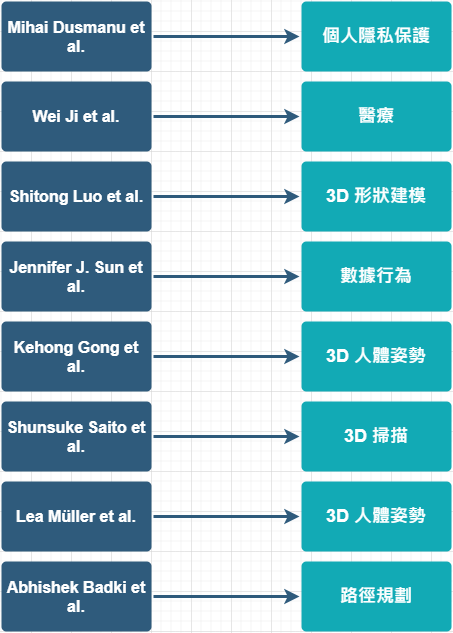
\includegraphics[width=0.60\textwidth]{m1.png} 
\caption{論文清單}
\label{Test}
\end{figure}

\section{Binary TTC}

接觸時間 (TTC),即物體與觀察者平面碰撞的時間,是路徑規劃的強大工具:它可能比場景中物體的深度、速度和加速度提供更多信息——即使對於人類也是如此。而 TTC 具有多種優勢,包括只需要一個單目、未校準的相機。然而,要做到回歸每個像素的 TTC 並不簡單,大多數現有方法對場景做出了過度簡化的假設。研究者們通過一系列更簡單的二元分類估計 TTC 來解決這一挑戰,他們以低延遲預測觀察者是否會在特定時間內與障礙物發生碰撞,這通常比知道精確的每像素 TTC 更重要。

對於這種情況,該研究的方法在 6.4 毫秒內提供了時間地理圍欄 (temporal geofence),此方法比現有方法快了 25 倍。當計算預算允許時,該研究的方法還可以通過任意精細的量化,包含連續值來估計每一個像素的 TTC。此方法是第一個以足夠高的幀速率提供 TTC 資訊 (binary or coarsely quantized) 以供實際使用的方法。

另外專案測試資料與包含論文中展示的測試結果整理如下。

\begin{figure}[H]
\centering  %圖片全局居中
\subfigure[測試 - img-ref.png]{
\label{Fig.sub.1}
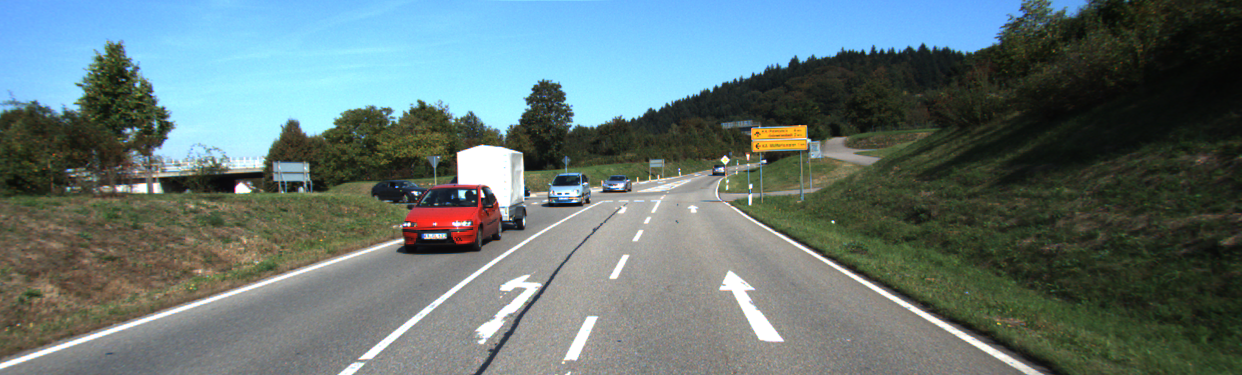
\includegraphics[width=0.45\textwidth]{img-ref.png}}
\subfigure[測試 - img-src.png]{
\label{Fig.sub.2}
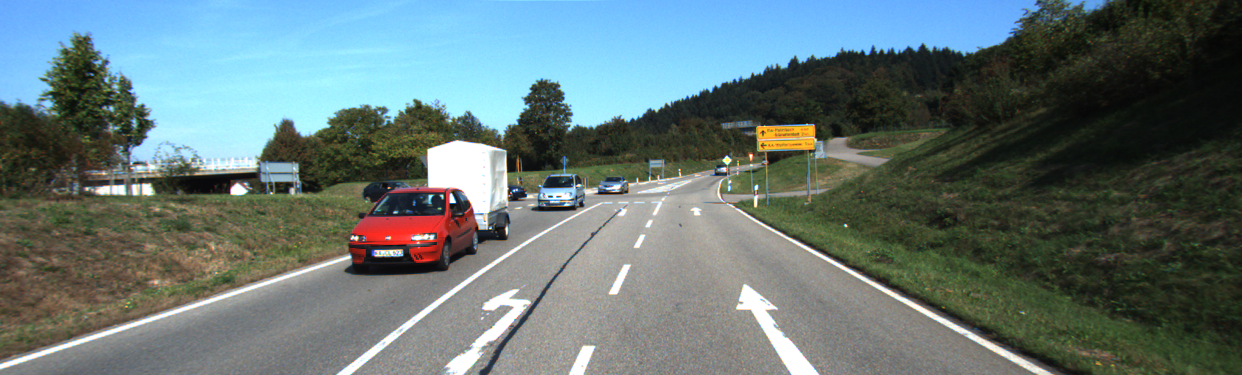
\includegraphics[width=0.45\textwidth]{img-src.png}}
\caption{測試論文資料}
\label{Fig.main}
\end{figure}

\begin{figure}[H]
\centering  %圖片全局居中
\subfigure[測試 - Reference image]{
\label{Fig.sub.1}
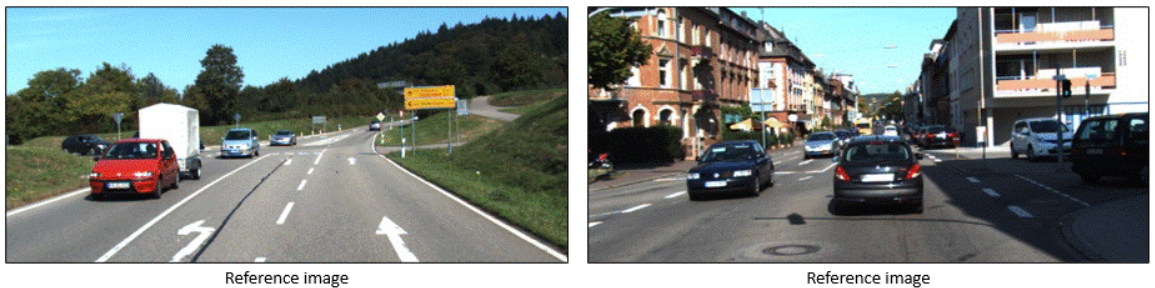
\includegraphics[width=0.45\textwidth]{t1.png}}
\subfigure[測試 - Source image]{
\label{Fig.sub.2}
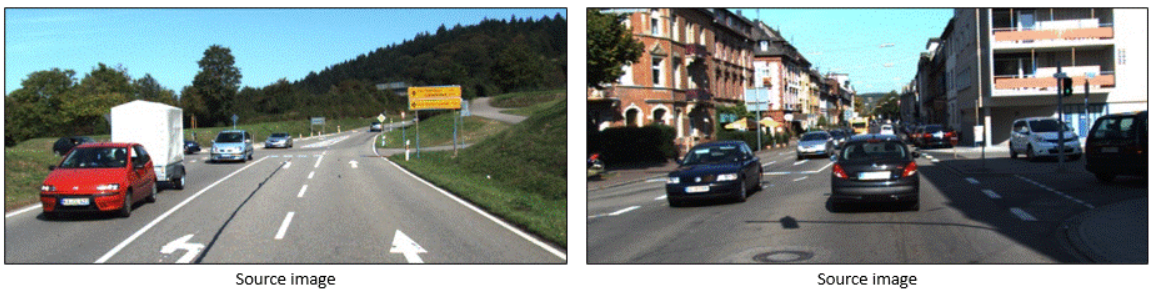
\includegraphics[width=0.45\textwidth]{t2.png}}
\subfigure[測試 - Binary TTC]{
\label{Fig.sub.3}
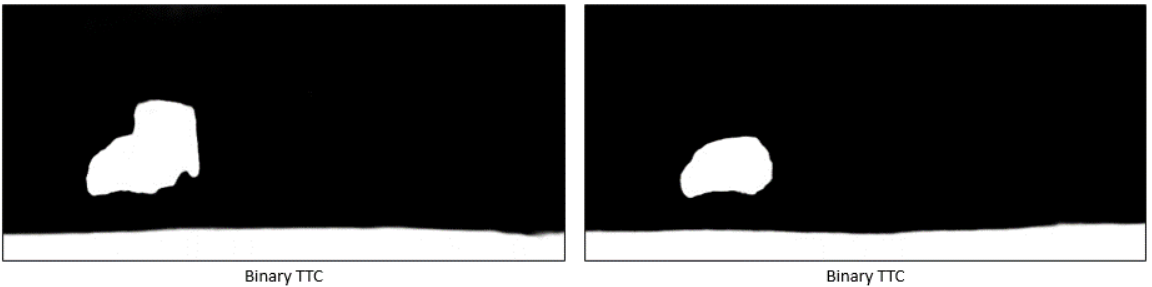
\includegraphics[width=0.45\textwidth]{t3.png}}
\subfigure[測試 - Quantized TTC]{
\label{Fig.sub.4}
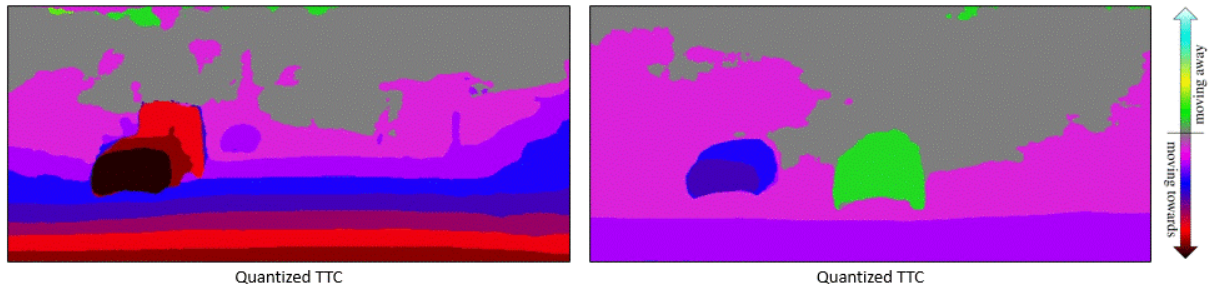
\includegraphics[width=0.45\textwidth]{t4.png}}
\subfigure[測試 - Continuous TTC]{
\label{Fig.sub.5}
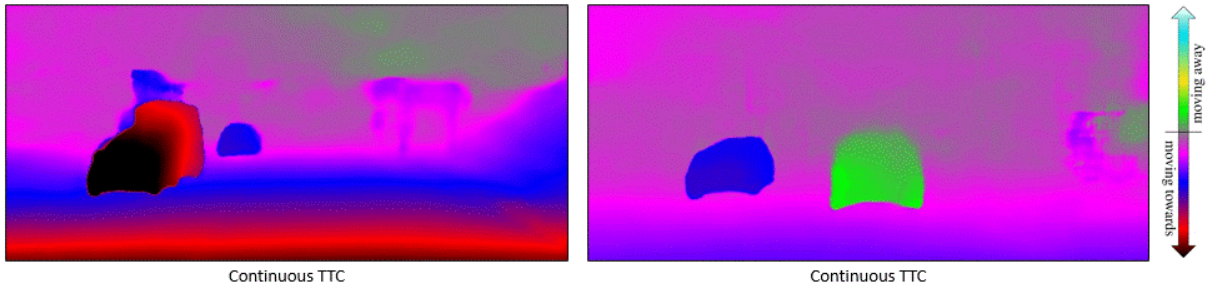
\includegraphics[width=0.45\textwidth]{t5.png}}
\caption{測試論文資料}
\label{Fig.main}
\end{figure}

\newpage

\section{Linux Shell 改寫成 PowerShell}

run\_continuous\_demo.sh 改寫成 run\_continuous\_demo.ps1。

\begin{lstlisting}[language={python}]
set CUDA_VISIBLE_DEVICES=1 ; python run_continuous_estimation.py `
    --attributes ttc of `
    --pretrained '../weights/cont_ttc_kitti15_trainval.pth.tar' `
    --alpha_min 0.5 `
    --alpha_max 1.3 `
    --alpha_size 18 `
    --shift_min -12 `
    --shift_max 12 `
    --shift_delta 1 `
    --bittcnet_crop_height 192 `
    --bittcnet_crop_width 576 `
    --ref_img_path '../data/img_ref.png' `
    --src_img_path '../data/img_src.png'
\end{lstlisting}

run\_binary\_demo.sh 改寫成 run\_binary\_demo.ps1。

\begin{lstlisting}[language={python}]
set CUDA_VISIBLE_DEVICES=1 ; python run_binary_estimation.py `
    --attribute ttc `
    --pretrained '../weights/binary_ttc_kitti15_train.pth.tar' `
    --fps 10 `
    --alpha_vals 0.7 0.75 0.8 0.85 0.9 0.95 0.98 1.02 1.10 `
    --ref_img_path '../data/img_ref.png' `
    --src_img_path '../data/img_src.png' 

set CUDA_VISIBLE_DEVICES=1 ; python run_binary_estimation.py `
    --attribute of `
    --pretrained '../weights/binary_ttc_kitti15_train.pth.tar' `
    --shifts_x -84 -64 -48 -36 -24 -12 0 12 24 36 48 64 84 `
    --shifts_y -36 -24 -12 0 6 12 18 24 30 48 60 72 84 `
    --ref_img_path '../data/img_ref.png' `
    --src_img_path '../data/img_src.png' 

\end{lstlisting}

\section{測試結果與 Demo}

%\begin{figure}[H]
%\centering  %圖片全局居中
%\subfigure[Sigmoid 函數]{
%\label{Fig.sub.1}
%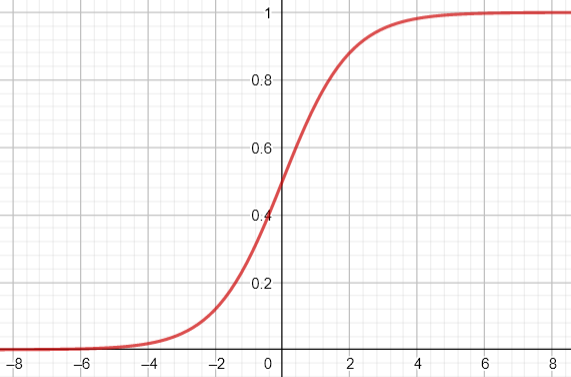
\includegraphics[width=0.45\textwidth]{mp1.png}}
%\subfigure[Sigmoid 函數求導與原函數對比]{
%\label{Fig.sub.2}
%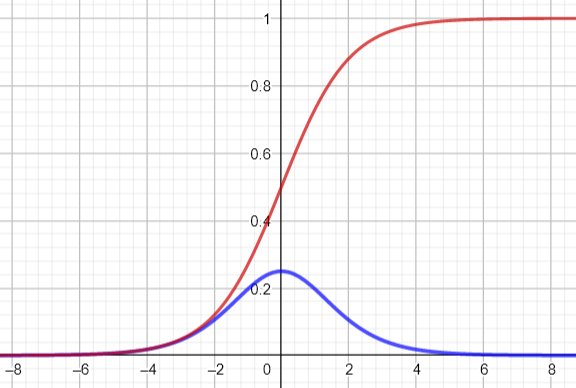
\includegraphics[width=0.45\textwidth]{mp2.png}}
%\caption{Sigmoid函數狀態}
%\label{Fig.main}
%\end{figure}

\begin{figure}[H]
\centering  %圖片全局居中
\subfigure[測試 - 000-thr0.70-img-in-0.jpg]{
\label{Fig.sub.1}
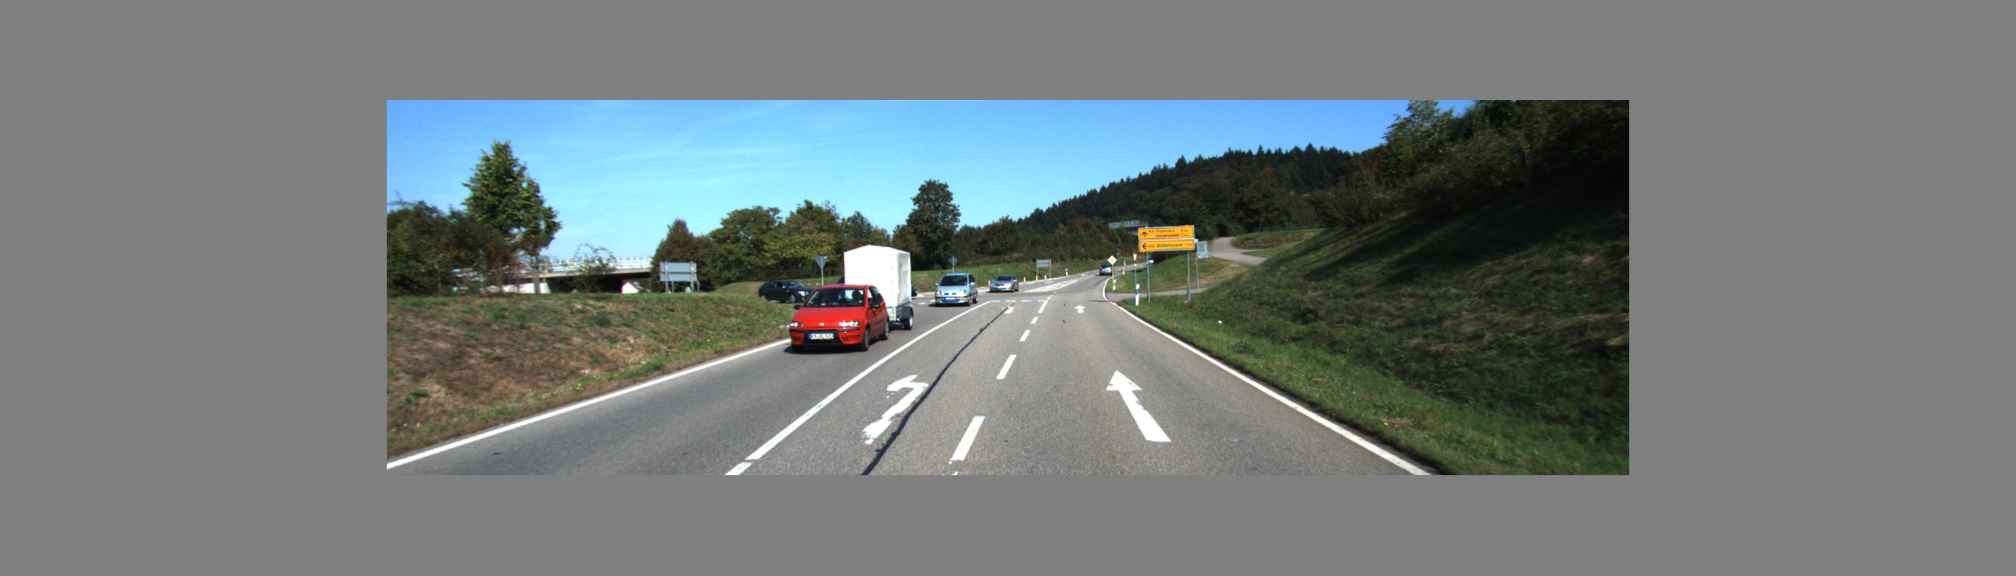
\includegraphics[width=0.3\textwidth]{000-thr0.70-img-in-0.jpg}}
\subfigure[測試 - 000-thr0.70-img-in-1.jpg]{
\label{Fig.sub.2}

\includegraphics[width=0.3\textwidth]{000-thr0.70-img-in-1.jpg}}
\subfigure[測試 - 000-thr0.70-seg-out.jpg]{
\label{Fig.sub.3}

\includegraphics[width=0.3\textwidth]{000-thr0.70-seg-out.jpg}}
\caption{000-thr0.70}
\label{Fig.main}
\end{figure}

\begin{figure}[H]
\centering  %圖片全局居中
\subfigure[測試 - 001-thr0.75-img-in-0.jpg]{
\label{Fig.sub.1}
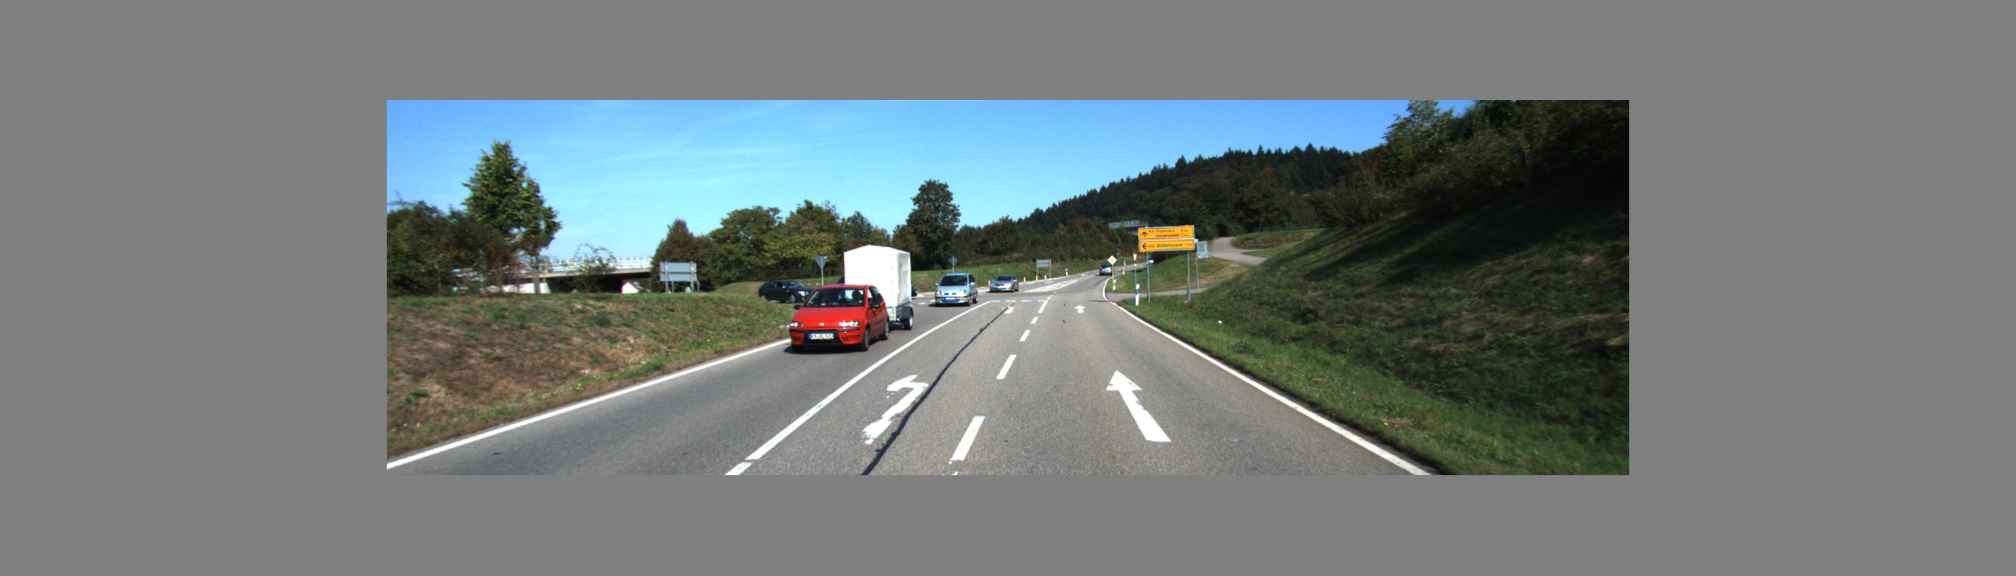
\includegraphics[width=0.3\textwidth]{001-thr0.75-img-in-0.jpg}}
\subfigure[測試 - 001-thr0.75-img-in-1.jpg]{
\label{Fig.sub.2}
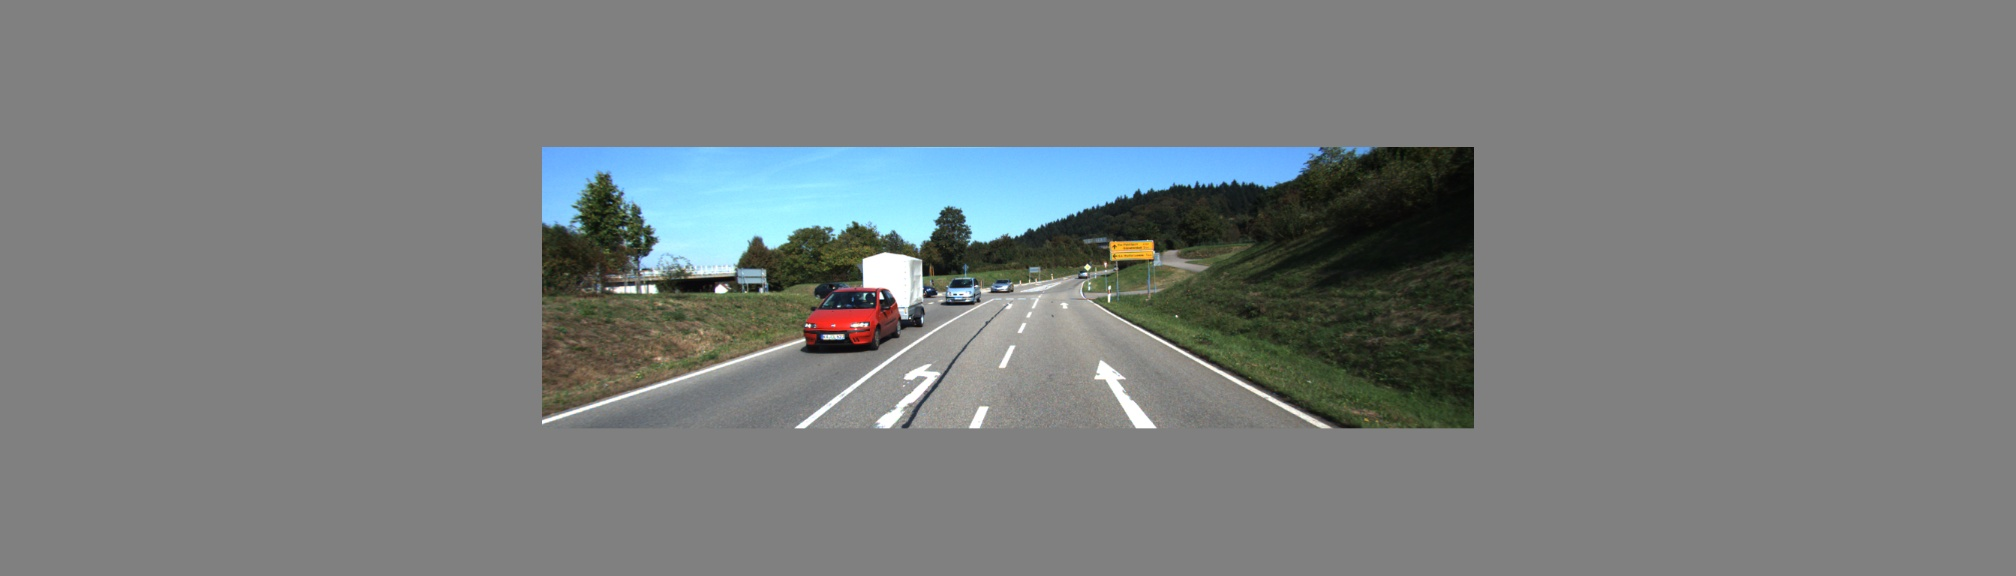
\includegraphics[width=0.3\textwidth]{001-thr0.75-img-in-1.jpg}}
\subfigure[測試 - 001-thr0.75-seg-out.jpg]{
\label{Fig.sub.3}

\includegraphics[width=0.3\textwidth]{001-thr0.75-seg-out.jpg}}
\caption{001-thr0.75}
\label{Fig.main}
\end{figure}

\begin{figure}[H]
\centering  %圖片全局居中
\subfigure[測試 - 002-thr0.80-img-in-0.jpg]{
\label{Fig.sub.1}
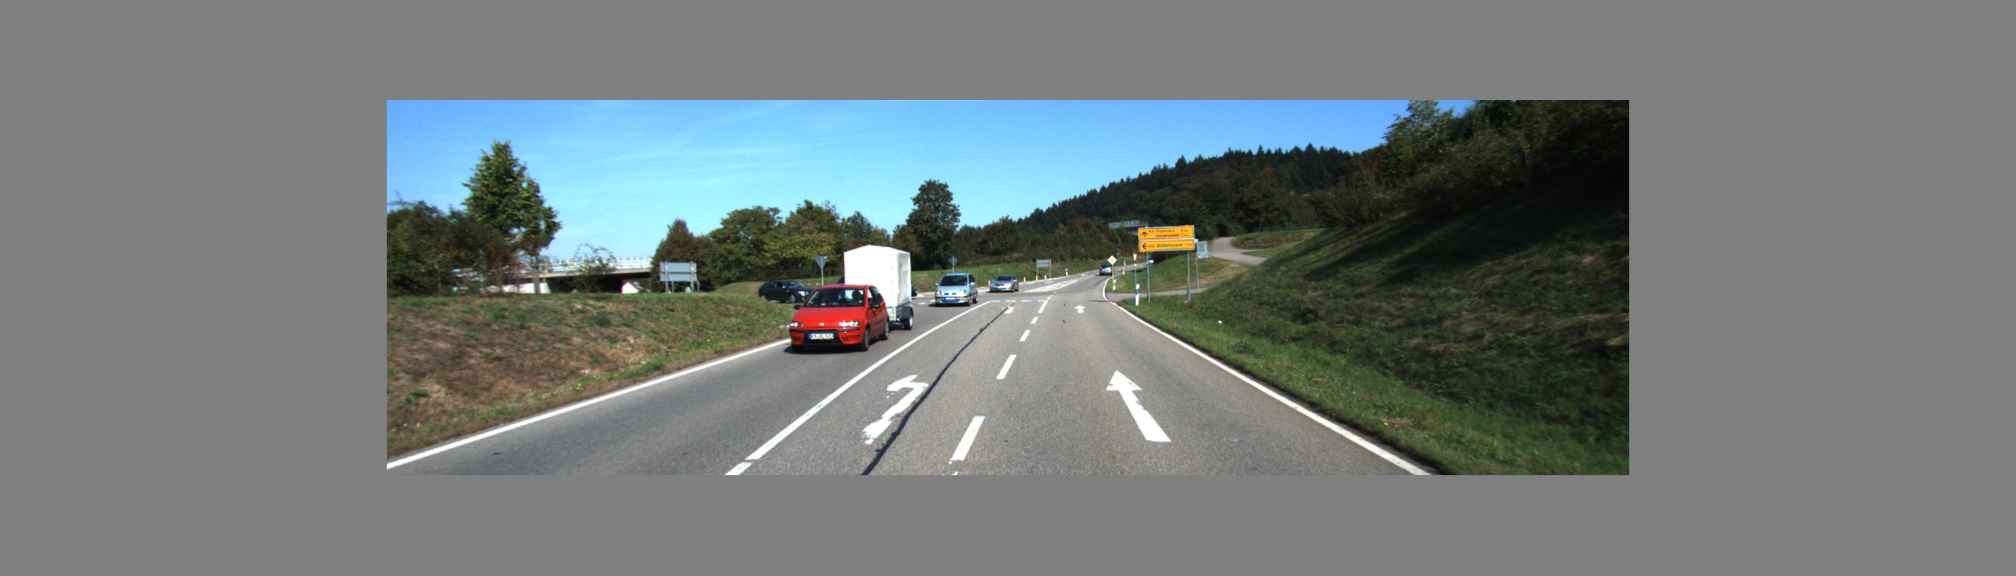
\includegraphics[width=0.3\textwidth]{002-thr0.80-img-in-0.jpg}}
\subfigure[測試 - 002-thr0.80-img-in-1.jpg]{
\label{Fig.sub.2}
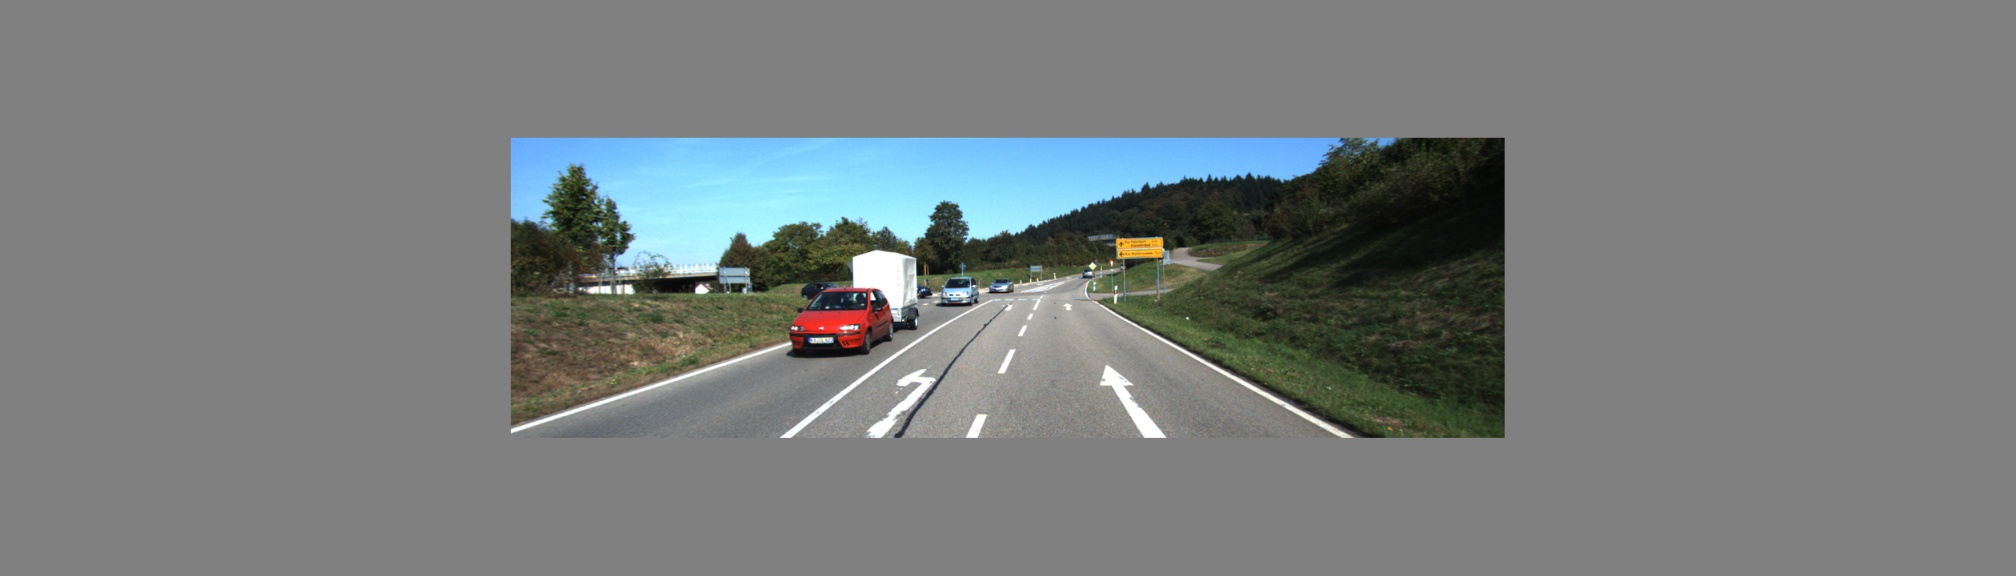
\includegraphics[width=0.3\textwidth]{002-thr0.80-img-in-1.jpg}}
\subfigure[測試 - 002-thr0.80-seg-out.jpg]{
\label{Fig.sub.3}

\includegraphics[width=0.3\textwidth]{002-thr0.80-seg-out.jpg}}
\caption{002-thr0.80}
\label{Fig.main}
\end{figure}

\begin{figure}[H]
\centering  %圖片全局居中
\subfigure[測試 - 003-thr0.85-img-in-0.jpg]{
\label{Fig.sub.1}
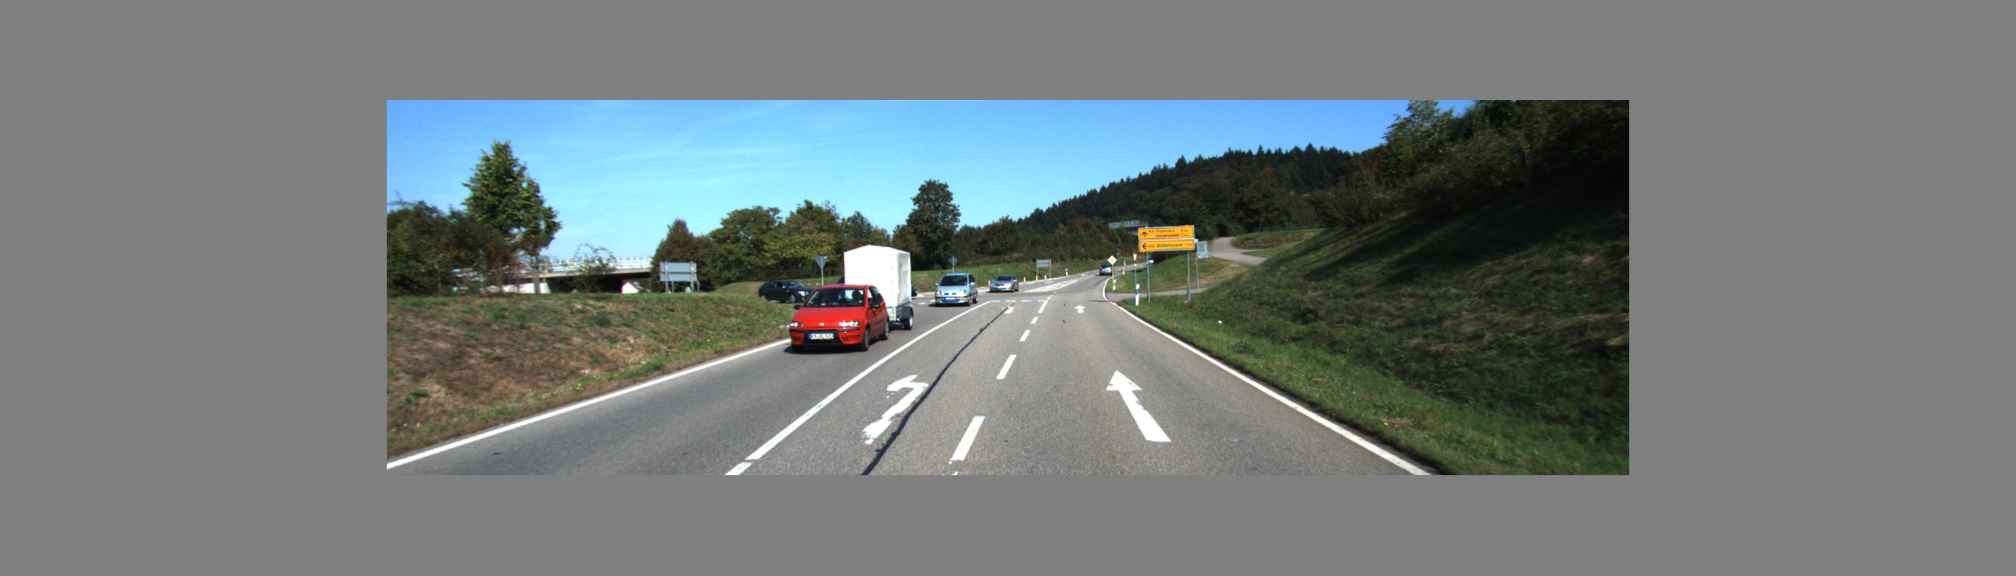
\includegraphics[width=0.3\textwidth]{003-thr0.85-img-in-0.jpg}}
\subfigure[測試 - 003-thr0.85-img-in-1.jpg]{
\label{Fig.sub.2}
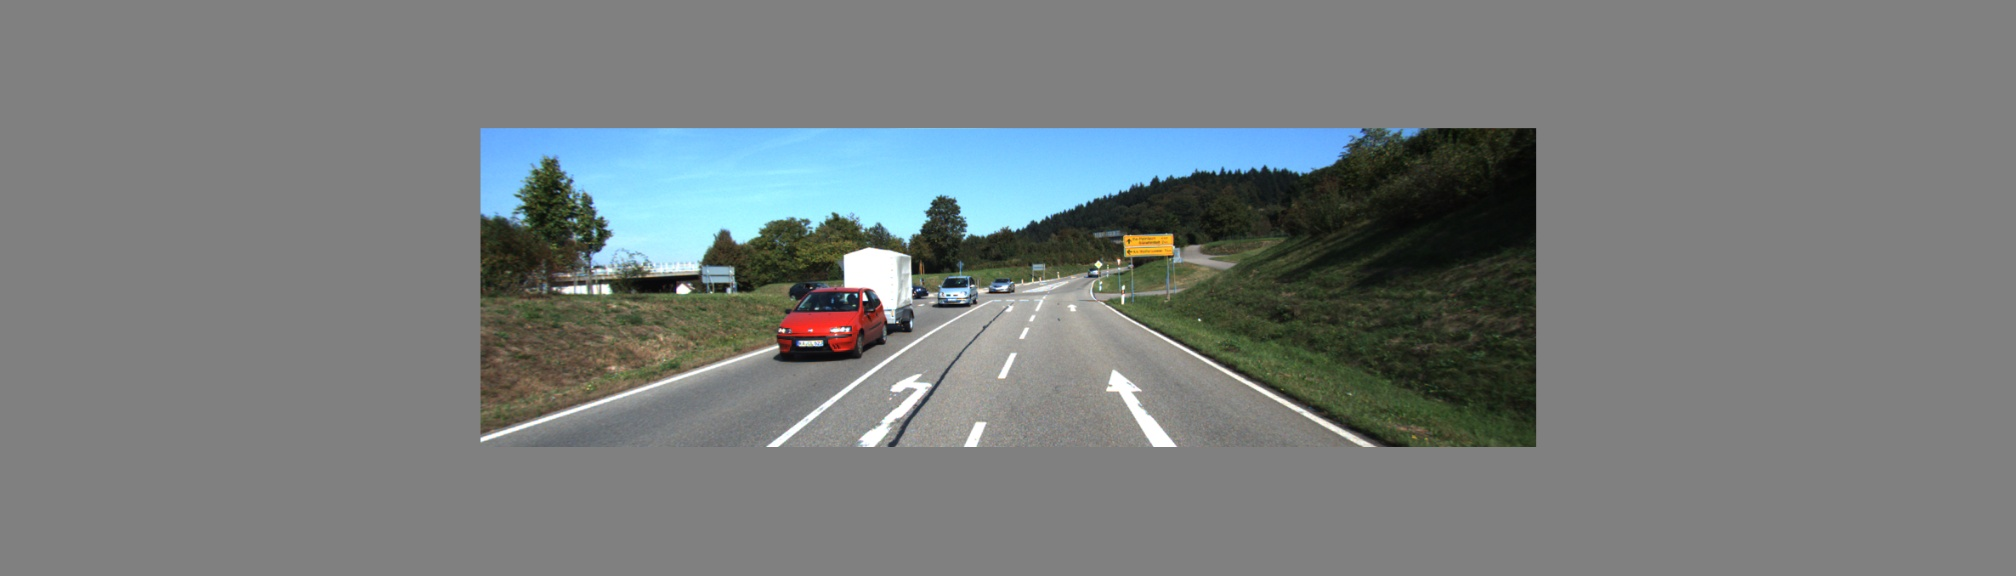
\includegraphics[width=0.3\textwidth]{003-thr0.85-img-in-1.jpg}}
\subfigure[測試 - 003-thr0.85-seg-out.jpg]{
\label{Fig.sub.3}

\includegraphics[width=0.3\textwidth]{003-thr0.85-seg-out.jpg}}
\caption{003-thr0.85}
\label{Fig.main}
\end{figure}

\begin{figure}[H]
\centering  %圖片全局居中
\subfigure[測試 - 004-thr0.90-img-in-0.jpg]{
\label{Fig.sub.1}
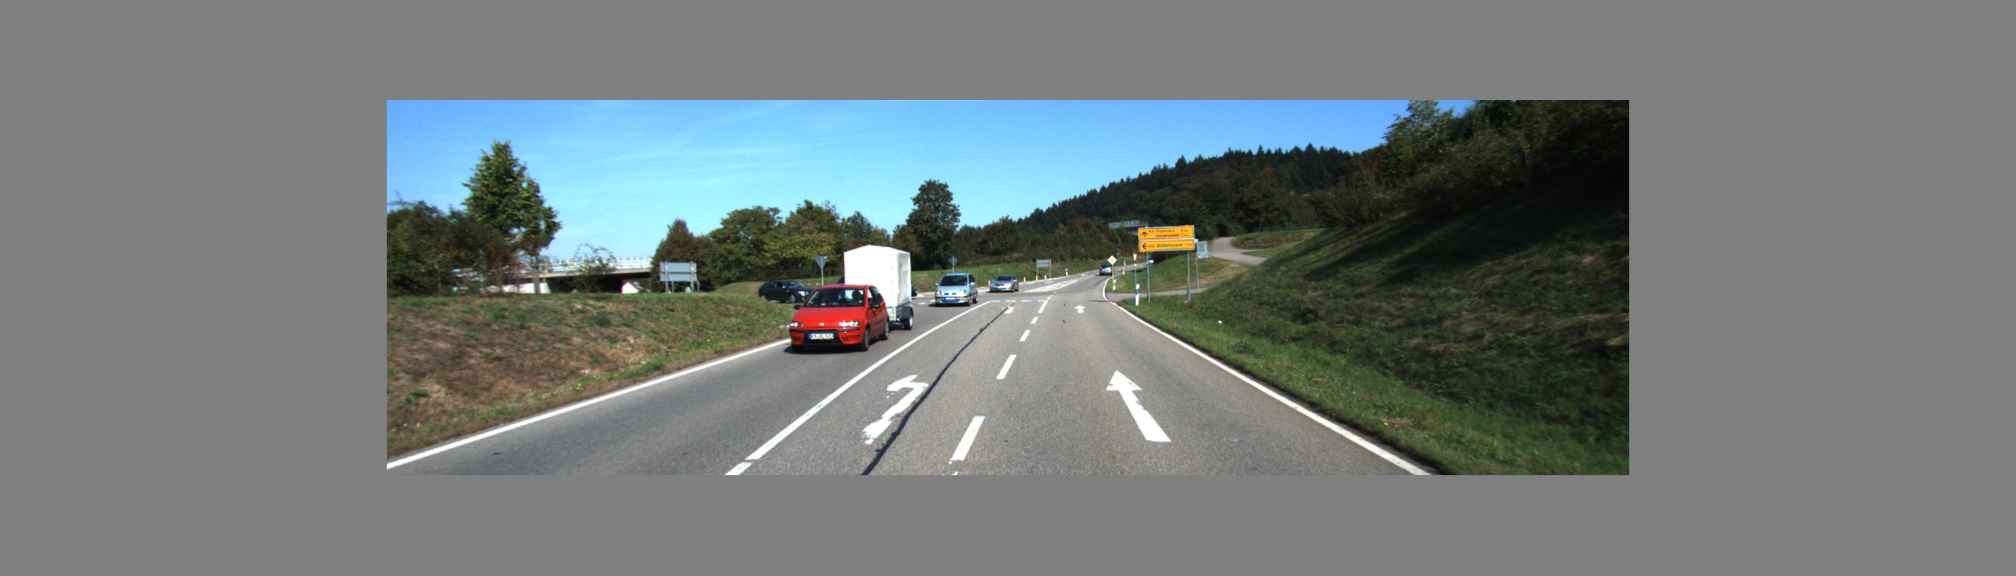
\includegraphics[width=0.3\textwidth]{004-thr0.90-img-in-0.jpg}}
\subfigure[測試 - 004-thr0.90-img-in-1.jpg]{
\label{Fig.sub.2}
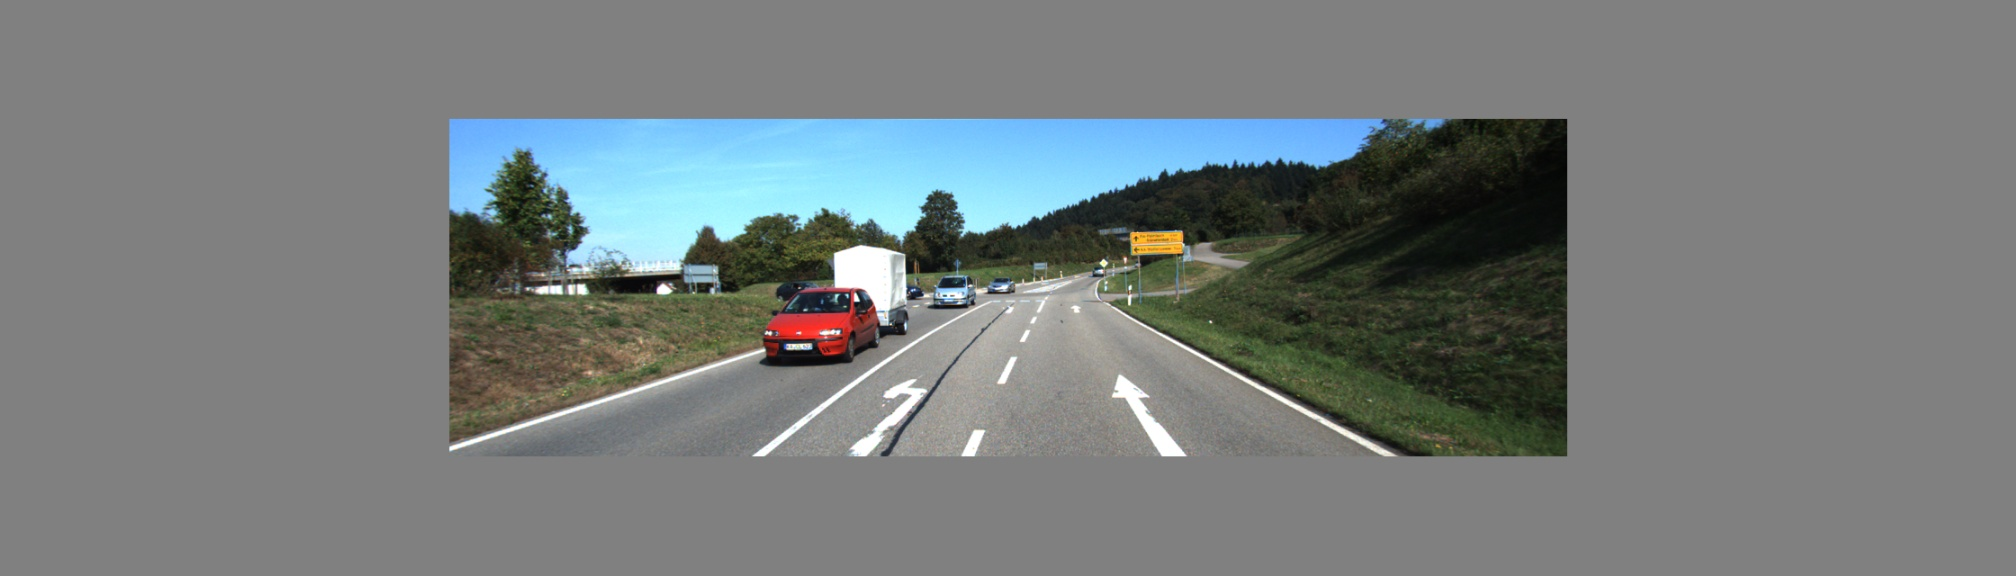
\includegraphics[width=0.3\textwidth]{004-thr0.90-img-in-1.jpg}}
\subfigure[測試 - 004-thr0.90-seg-out.jpg]{
\label{Fig.sub.3}

\includegraphics[width=0.3\textwidth]{004-thr0.90-seg-out.jpg}}
\caption{004-thr0.90}
\label{Fig.main}
\end{figure}

\begin{figure}[H]
\centering  %圖片全局居中
\subfigure[測試 - 005-thr0.95-img-in-0.jpg]{
\label{Fig.sub.1}
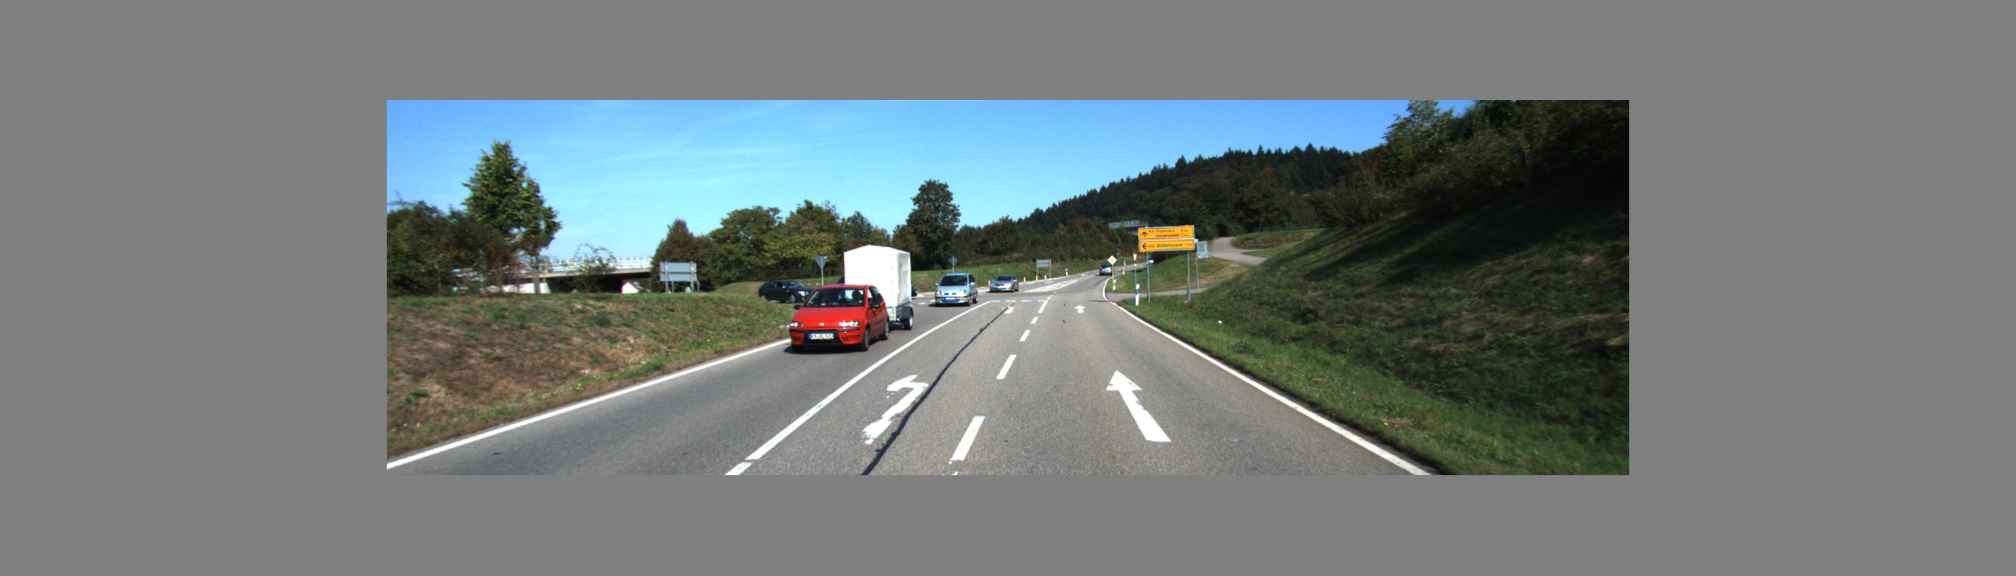
\includegraphics[width=0.3\textwidth]{005-thr0.95-img-in-0.jpg}}
\subfigure[測試 - 005-thr0.95-img-in-1.jpg]{
\label{Fig.sub.2}
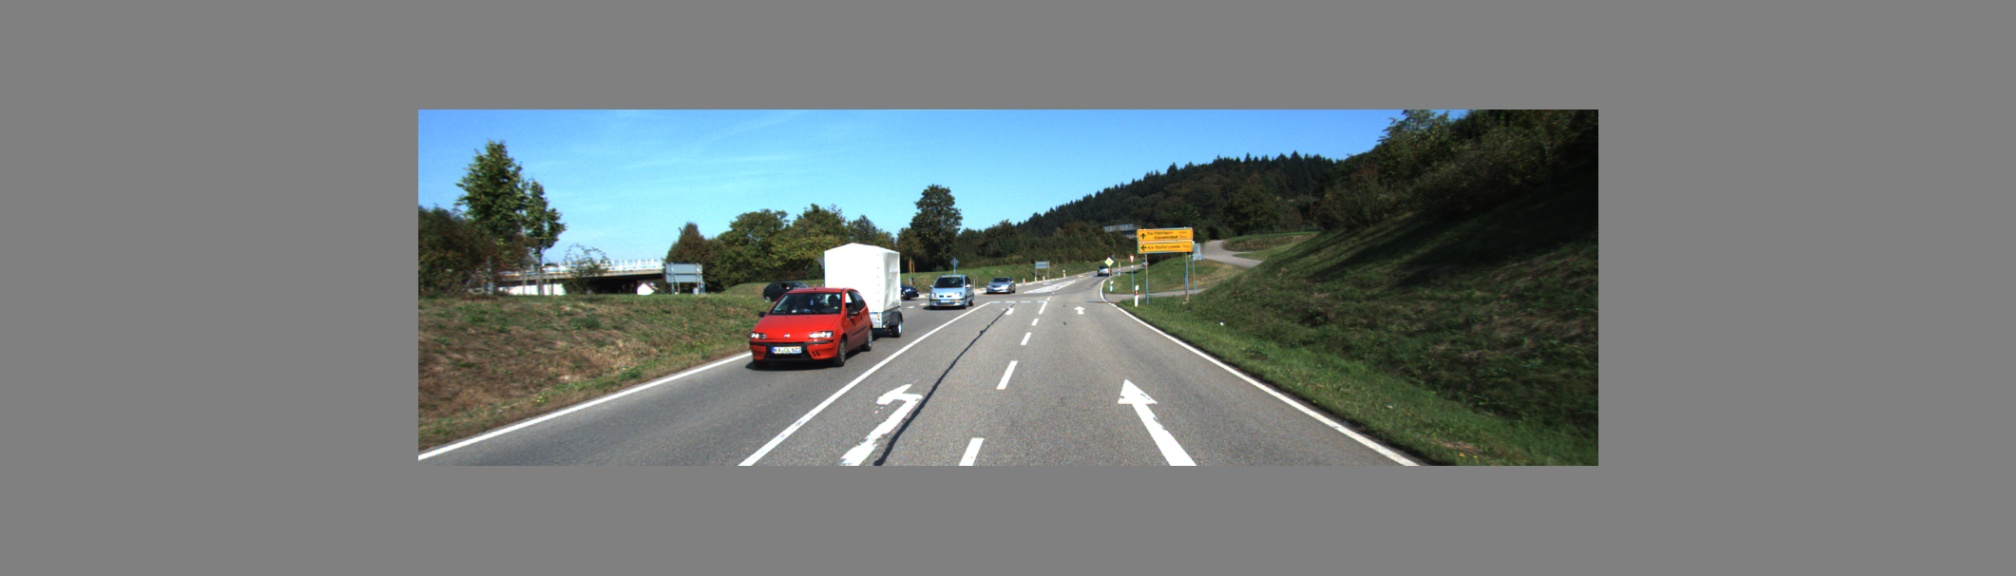
\includegraphics[width=0.3\textwidth]{005-thr0.95-img-in-1.jpg}}
\subfigure[測試 - 005-thr0.95-seg-out.jpg]{
\label{Fig.sub.3}
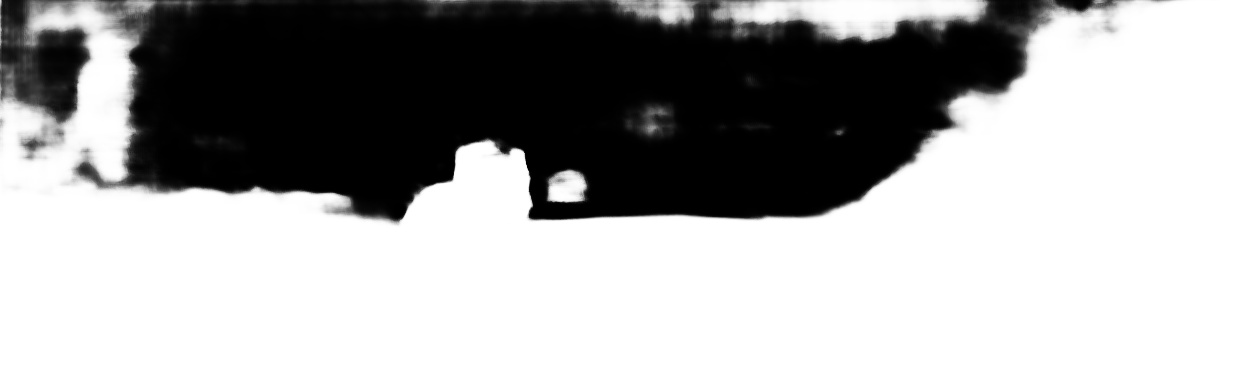
\includegraphics[width=0.3\textwidth]{005-thr0.95-seg-out.jpg}}
\caption{005-thr0.95}
\label{Fig.main}
\end{figure}

\begin{figure}[H]
\centering  %圖片全局居中
\subfigure[測試 - 006-thr0.98-img-in-0.jpg]{
\label{Fig.sub.1}
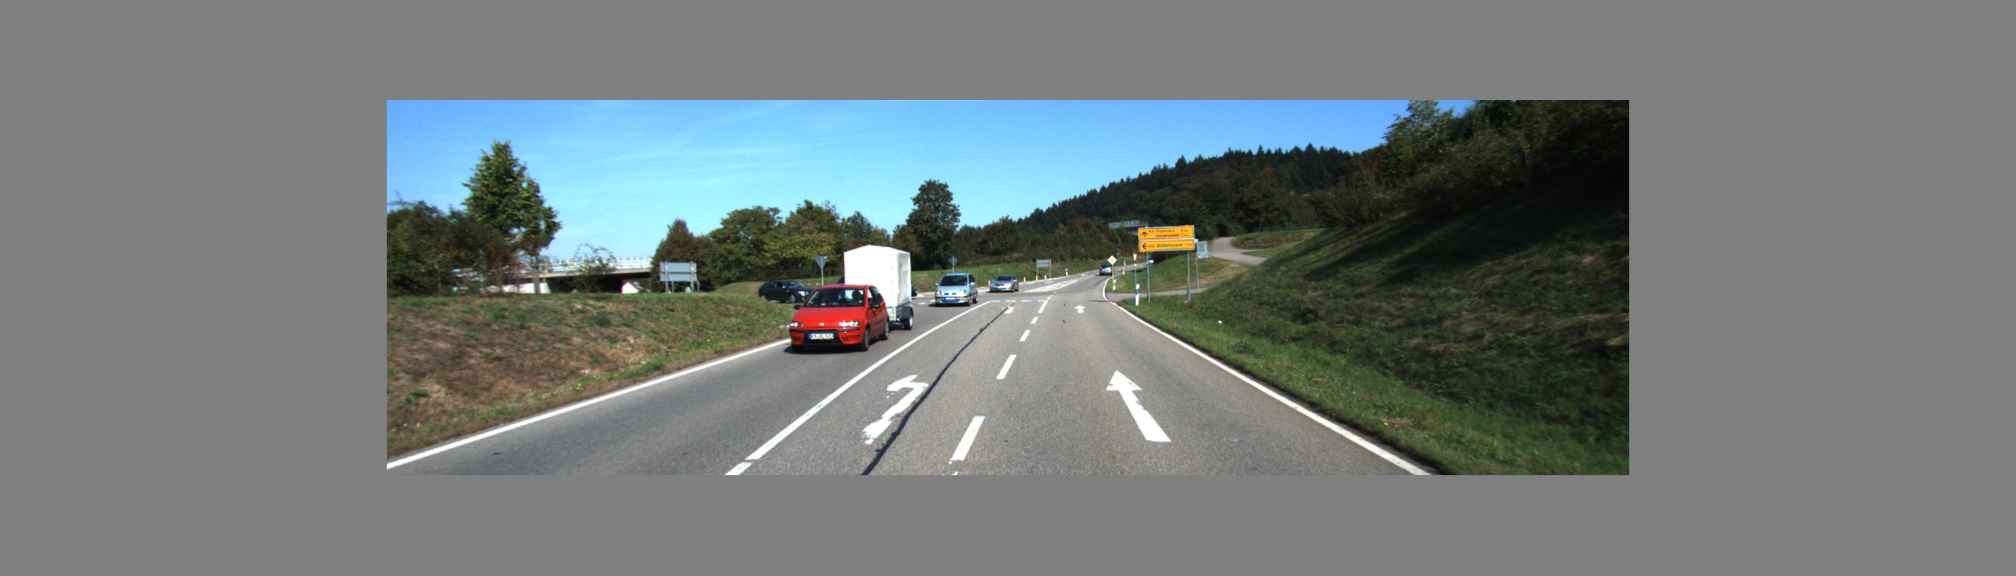
\includegraphics[width=0.3\textwidth]{006-thr0.98-img-in-0.jpg}}
\subfigure[測試 - 006-thr0.98-img-in-1.jpg]{
\label{Fig.sub.2}
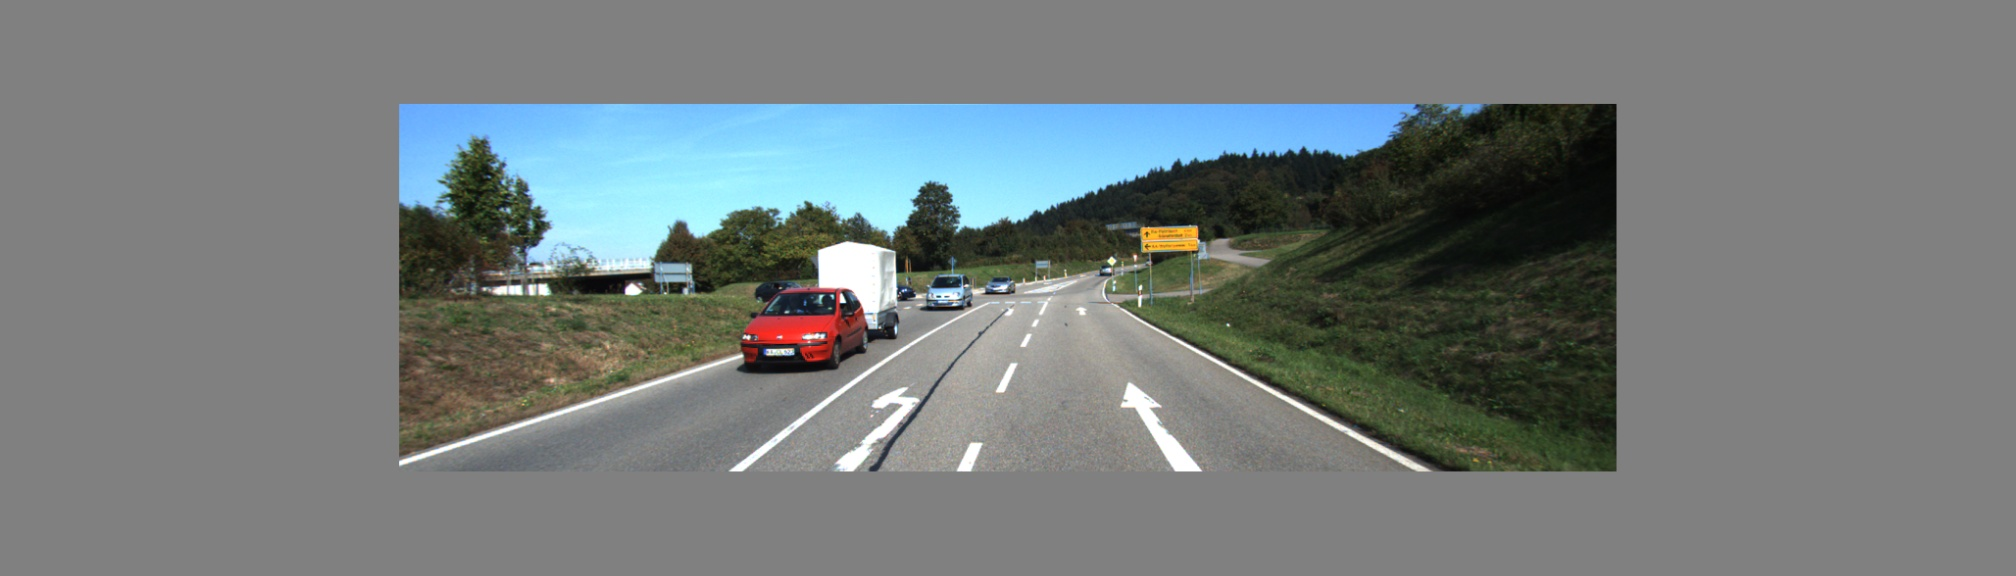
\includegraphics[width=0.3\textwidth]{006-thr0.98-img-in-1.jpg}}
\subfigure[測試 - 006-thr0.98-seg-out.jpg]{
\label{Fig.sub.3}
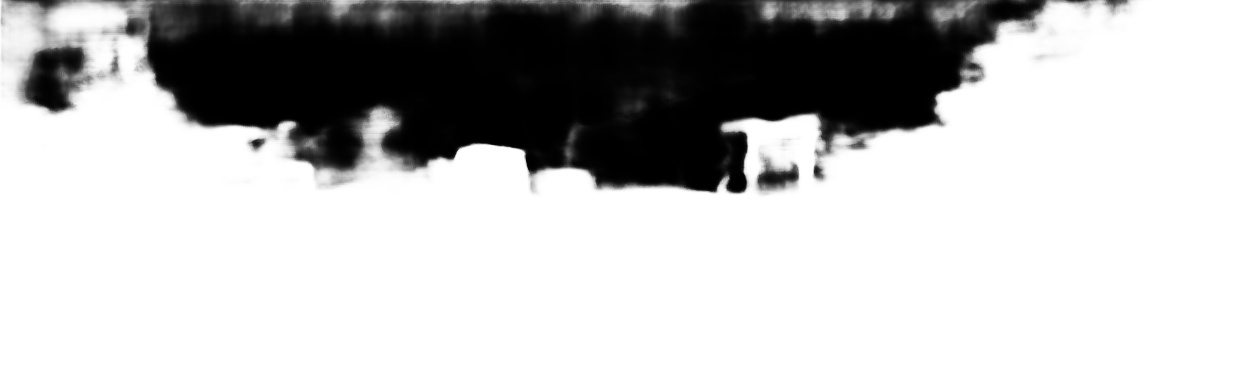
\includegraphics[width=0.3\textwidth]{006-thr0.98-seg-out.jpg}}
\caption{006-thr0.98}
\label{Fig.main}
\end{figure}

\begin{figure}[H]
\centering  %圖片全局居中
\subfigure[測試 - 007-thr1.02-img-in-0.jpg]{
\label{Fig.sub.1}
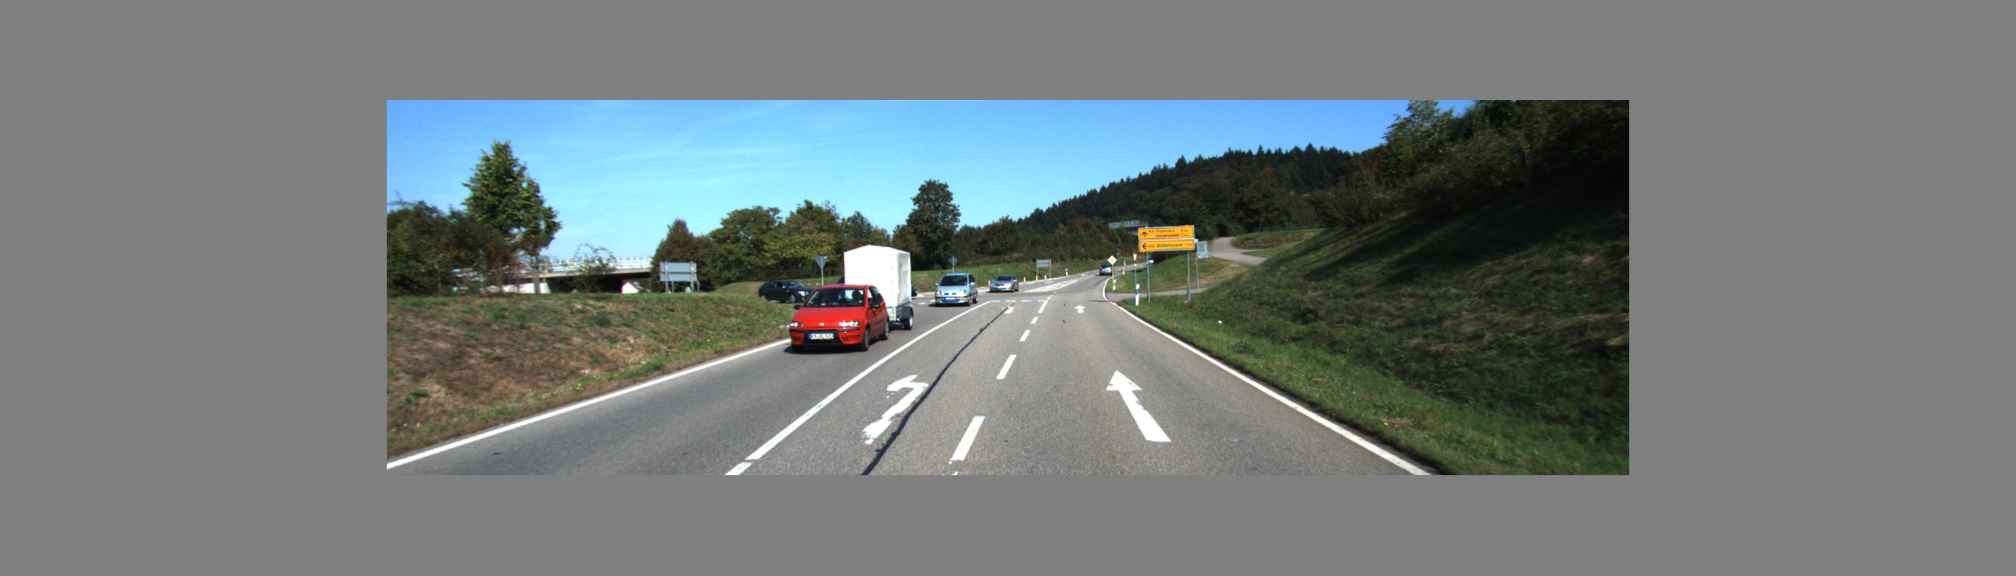
\includegraphics[width=0.3\textwidth]{007-thr1.02-img-in-0.jpg}}
\subfigure[測試 - 007-thr1.02-img-in-1.jpg]{
\label{Fig.sub.2}
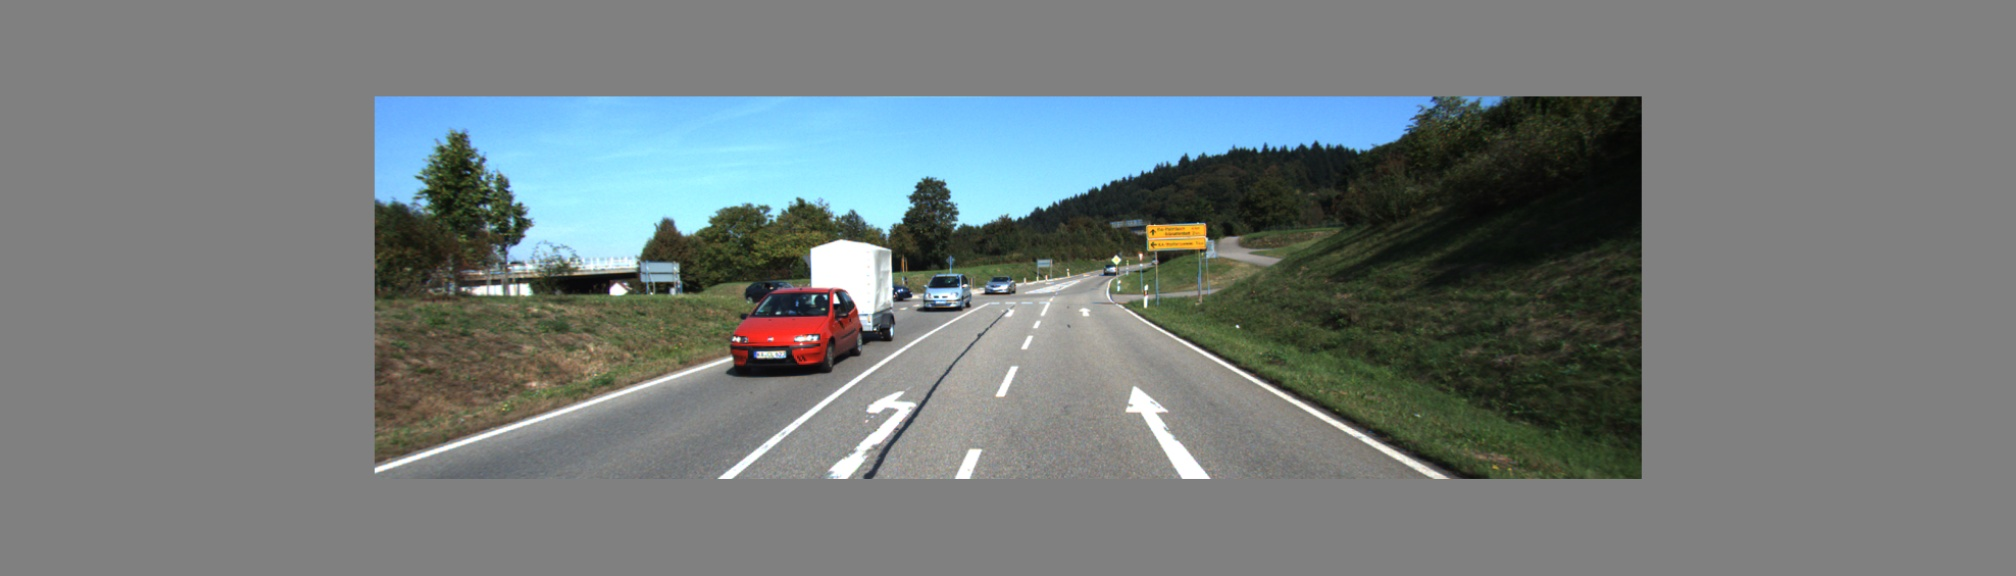
\includegraphics[width=0.3\textwidth]{007-thr1.02-img-in-1.jpg}}
\subfigure[測試 - 007-thr1.02-seg-out.jpg]{
\label{Fig.sub.3}

\includegraphics[width=0.3\textwidth]{007-thr1.02-seg-out.jpg}}
\caption{007-thr1.02}
\label{Fig.main}
\end{figure}

\begin{figure}[H]
\centering  %圖片全局居中
\subfigure[測試 - 008-thr1.10-img-in-0.jpg]{
\label{Fig.sub.1}
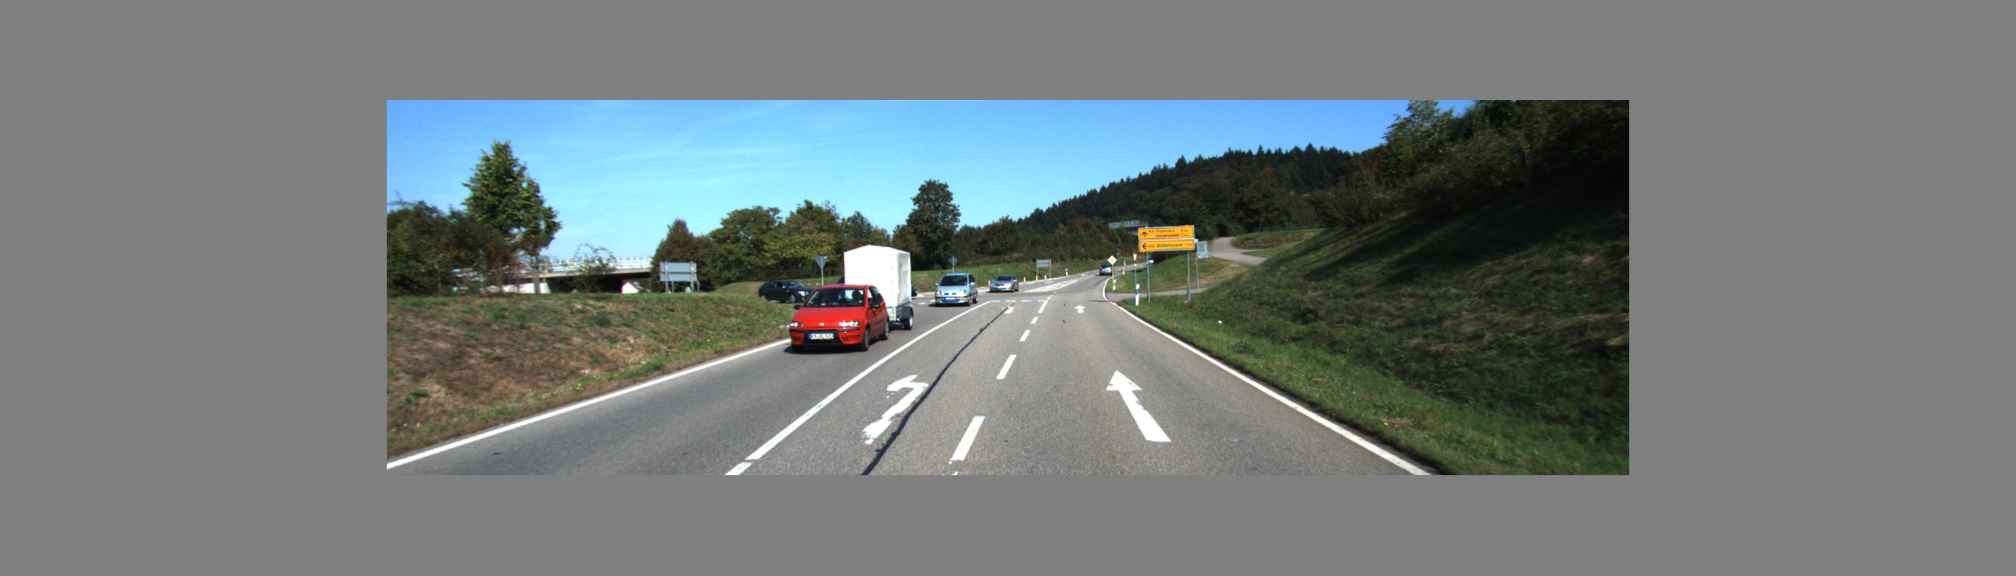
\includegraphics[width=0.3\textwidth]{008-thr1.10-img-in-0.jpg}}
\subfigure[測試 - 008-thr1.10-img-in-1.jpg]{
\label{Fig.sub.2}
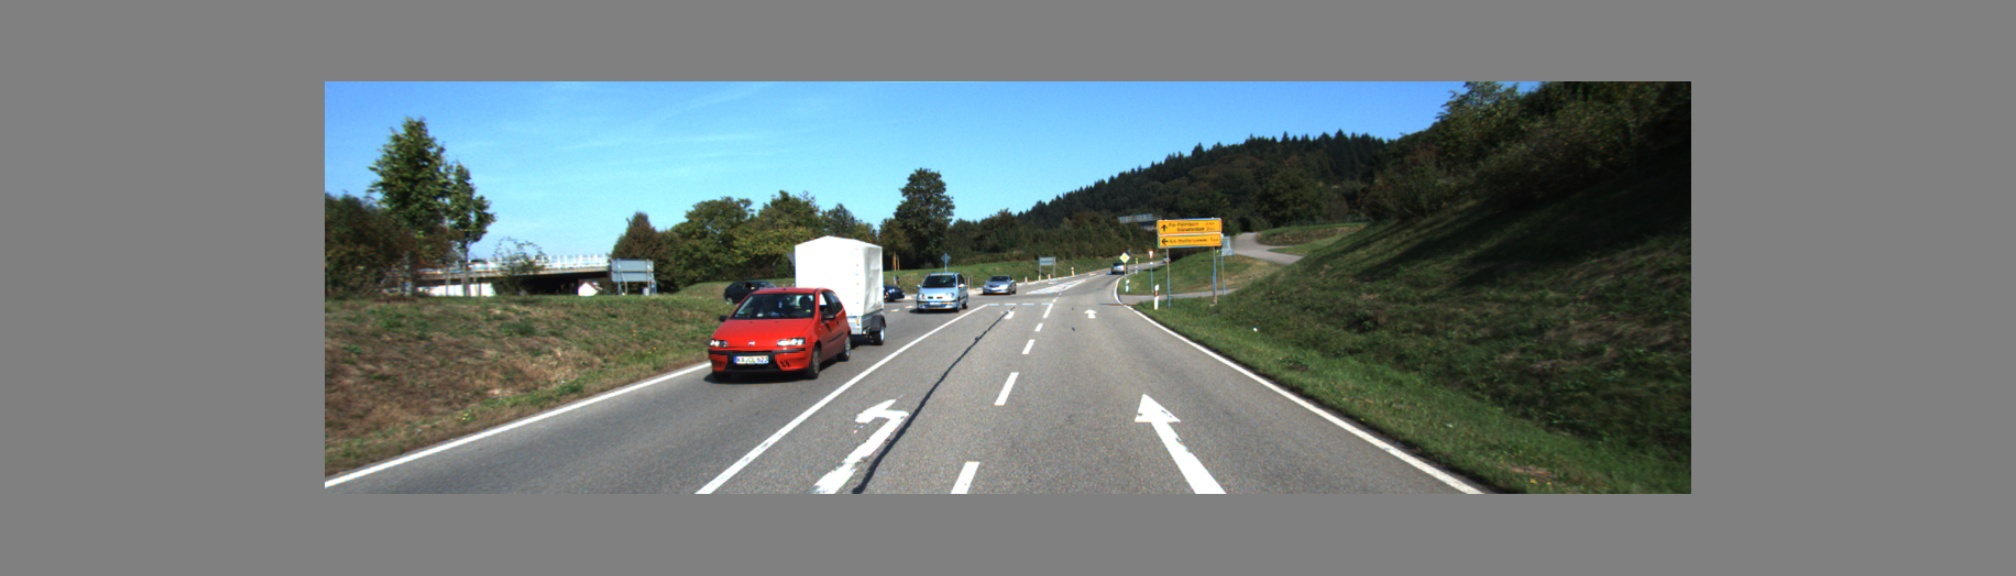
\includegraphics[width=0.3\textwidth]{008-thr1.10-img-in-1.jpg}}
\subfigure[測試 - 008-thr1.10-seg-out.jpg]{
\label{Fig.sub.3}

\includegraphics[width=0.3\textwidth]{008-thr1.10-seg-out.jpg}}
\caption{008-thr1.10}
\label{Fig.main}
\end{figure}

\begin{figure}[H]
\centering 

\includegraphics[width=0.60\textwidth]{quant-ttc-out.jpg} 
\caption{quant-ttc-out.jpg}
\label{Test}
\end{figure}

\begin{figure}[H]
\centering  %圖片全局居中
\subfigure[測試 - eta-out.png]{
\label{Fig.sub.1}

\includegraphics[width=0.45\textwidth]{eta-out.png}}
\subfigure[測試 - of-out.png]{
\label{Fig.sub.2}

\includegraphics[width=0.45\textwidth]{of-out.png}}
\caption{cont\_ttc-of}
\label{Fig.main}
\end{figure}

\newpage

\section{附件}

執行 run\_continuous\_demo.ps1 的結果。

\begin{verbatim}
(bittc) PS D:\py-test\BiTTC-master\test\src> .\run_continuous_demo.ps1
==> ALL PARAMETERS
ref_img_path : ../data/img_ref.png
src_img_path : ../data/img_src.png
attributes : ['ttc', 'of']
pretrained : ../weights/cont_ttc_kitti15_trainval.pth.tar
arch : bittcnet_continuous_of_ttc_2d
bittcnet_featnet_arch : featextractnetspp
bittcnet_segnet_arch : segnet2d
segnet_num_imgs : 2
segnet_num_segs : 3
segnet_is_deep : True
regrefinenet_out_planes : 32
bittcnet_max_scale : 1.5
alpha_min : 0.5
alpha_max : 1.3
alpha_size : 18
shift_min : -12.0
shift_max : 12.0
shift_delta : 1
bittcnet_crop_height : 192
bittcnet_crop_width : 576
dtype : torch.float32
device : cuda

Results will be dumped in ./results/21_11_30-00_31_21_cont_ttc-of

Padding will be added to ensure input image size divisible by 192
New input image size is 384 x 1344
Crop size will be 192 x 576
=> using pre-trained model 'bittcnet_continuous_of_ttc_2d'
==> USING BiTTCNetContinuousOFTTC2D
bittcnet_featnet_arch : featextractnetspp
bittcnet_segnet_arch : segnet2d
bittcnet_max_scale : 1.5
bittcnet_crop_height : 192
bittcnet_crop_width : 576
bittcnet_full_height : 384
bittcnet_full_width : 1344
==> USING FeatExtractNetSPP
bittcnet_featnet_arch : featextractnetspp
==> USING SegNet2D
==> USING RegRefineNet
regrefinenet_out_planes : 32
C:\Users\zxdfg\.conda\envs\bittc\lib\site-packages\torch\nn\functional.py:4003: UserWarning: Default grid_sample and affine_grid behavior has changed to align_corners=False since 1.3.0. Please specify align_corners=True if the old behavior is desired. See the documentation of grid_sample for details.
  warnings.warn(

Results generated

Visualizing results

DONE!
\end{verbatim}

執行 run\_binary\_demo.ps1 的結果。

\begin{verbatim}
(bittc) PS D:\py-test\BiTTC-master\test\src> .\run_binary_demo.ps1
==> ALL PARAMETERS
ref_img_path : ../data/img_ref.png
src_img_path : ../data/img_src.png
attribute : ttc
pretrained : ../weights/binary_ttc_kitti15_train.pth.tar
arch : bittcnet_binary_of_ttc_2d
bittcnet_featnet_arch : featextractnetspp
bittcnet_featnethr_arch : featextractnethr
bittcnet_segnet_arch : segnet2d
bittcnet_refinenet_arch : segrefinenet
segnet_num_imgs : 2
segnet_num_segs : 3
bittcnet_num_refinenets : 3
featextractnethr_out_planes : 16
segrefinenet_in_planes : 17
segrefinenet_out_planes : 8
segrefinenet_num_layers : 4
bittcnet_max_scale : 1.5
alpha_vals : [0.7, 0.75, 0.8, 0.85, 0.9, 0.95, 0.98, 1.02, 1.1]
shifts_x : [-72, -60, -48, -36, -24, -12, 0, 12, 24, 36, 48, 60, 72]
shifts_y : [-18, -15, -12, -9, -6, -3, 0, 3, 6, 9, 12, 15, 18]
fps : 10.0
dtype : torch.float32
device : cuda

Results will be dumped in ./results/21_11_30-00_31_32_binary_ttc

Padding will be added to ensure input image size divisible by 192
New input image size is 384 x 1344


Computing binary TTC

alpha/motion-in-depth threshold values:
[0.7  0.75 0.8  0.85 0.9  0.95 0.98 1.02 1.1 ]

corresponding time-to-contact threshould values:
[ 0.33333334  0.4         0.50000006  0.6666668   0.9999998   1.9999996
  5.0000052  -5.0000052  -0.9999998 ]

=> using pre-trained model 'bittcnet_binary_of_ttc_2d'
==> USING BiTTCNetBinaryOFTTC2D
bittcnet_featnet_arch : featextractnetspp
bittcnet_featnethr_arch : featextractnethr
bittcnet_segnet_arch : segnet2d
bittcnet_refinenet_arch : segrefinenet
bittcnet_num_refinenets : 3
bittcnet_max_scale : 1.5
bittcnet_crop_height : 384
bittcnet_crop_width : 1344
==> USING FeatExtractNetSPP
bittcnet_featnet_arch : featextractnetspp
bittcnet_featnethr_arch : featextractnethr
featextractnethr_out_planes : 16
==> USING SegNet2D
==> USING FeatExtractNetHR
featextractnethr_out_planes : 16
==> USING SegRefineNet
segrefinenet_in_planes : 17
segrefinenet_out_planes : 8
segrefinenet_num_layers : 4
==> USING SegRefineNet
segrefinenet_in_planes : 17
segrefinenet_out_planes : 8
segrefinenet_num_layers : 4
==> USING SegRefineNet
segrefinenet_in_planes : 17
segrefinenet_out_planes : 8
segrefinenet_num_layers : 4
C:\Users\zxdfg\.conda\envs\bittc\lib\site-packages\torch\nn\functional.py:4003: UserWarning: Default grid_sample and affine_grid behavior has changed to align_corners=False since 1.3.0. Please specify align_corners=True if the old behavior is desired. See the documentation of grid_sample for details.
  warnings.warn(

Results generated

Visualizing results

alpha threshold values are in increasing order
Computing quantized TTC map

DONE!
==> ALL PARAMETERS
ref_img_path : ../data/img_ref.png
src_img_path : ../data/img_src.png
attribute : of
pretrained : ../weights/binary_ttc_kitti15_train.pth.tar
arch : bittcnet_binary_of_ttc_2d
bittcnet_featnet_arch : featextractnetspp
bittcnet_featnethr_arch : featextractnethr
bittcnet_segnet_arch : segnet2d
bittcnet_refinenet_arch : segrefinenet
segnet_num_imgs : 2
segnet_num_segs : 3
bittcnet_num_refinenets : 3
featextractnethr_out_planes : 16
segrefinenet_in_planes : 17
segrefinenet_out_planes : 8
segrefinenet_num_layers : 4
bittcnet_max_scale : 1.5
alpha_vals : [0.7, 0.75, 0.8, 0.85, 0.9, 0.95, 0.98, 1.02, 1.1]
shifts_x : [-84.0, -64.0, -48.0, -36.0, -24.0, -12.0, 0.0, 12.0, 24.0, 36.0, 48.0, 64.0, 84.0]
shifts_y : [-36.0, -24.0, -12.0, 0.0, 6.0, 12.0, 18.0, 24.0, 30.0, 48.0, 60.0, 72.0, 84.0]
fps : 10
dtype : torch.float32
device : cuda

Results will be dumped in ./results/21_11_30-00_31_40_binary_of

Padding will be added to ensure input image size divisible by 192
New input image size is 384 x 1344


Computing 2D binary OF

2D Binary optical flow segmentation will be computed with respect to following thresholds:
(-84.00, -36.00)
(-64.00, -24.00)
(-48.00, -12.00)
(-36.00, 0.00)
(-24.00, 6.00)
(-12.00, 12.00)
(0.00, 18.00)
(12.00, 24.00)
(24.00, 30.00)
(36.00, 48.00)
(48.00, 60.00)
(64.00, 72.00)
(84.00, 84.00)

=> using pre-trained model 'bittcnet_binary_of_ttc_2d'
==> USING BiTTCNetBinaryOFTTC2D
bittcnet_featnet_arch : featextractnetspp
bittcnet_featnethr_arch : featextractnethr
bittcnet_segnet_arch : segnet2d
bittcnet_refinenet_arch : segrefinenet
bittcnet_num_refinenets : 3
bittcnet_max_scale : 1.5
bittcnet_crop_height : 384
bittcnet_crop_width : 1344
==> USING FeatExtractNetSPP
bittcnet_featnet_arch : featextractnetspp
bittcnet_featnethr_arch : featextractnethr
featextractnethr_out_planes : 16
==> USING SegNet2D
==> USING FeatExtractNetHR
featextractnethr_out_planes : 16
==> USING SegRefineNet
segrefinenet_in_planes : 17
segrefinenet_out_planes : 8
segrefinenet_num_layers : 4
==> USING SegRefineNet
segrefinenet_in_planes : 17
segrefinenet_out_planes : 8
segrefinenet_num_layers : 4
==> USING SegRefineNet
segrefinenet_in_planes : 17
segrefinenet_out_planes : 8
segrefinenet_num_layers : 4
C:\Users\zxdfg\.conda\envs\bittc\lib\site-packages\torch\nn\functional.py:4003: UserWarning: Default grid_sample and affine_grid behavior has changed to align_corners=False since 1.3.0. Please specify align_corners=True if the old behavior is desired. See the documentation of grid_sample for details.
  warnings.warn(
Traceback (most recent call last):
  File "D:\py-test\BiTTC-master\test\src\run_binary_estimation.py", line 326, in <module>
    main()
  File "D:\py-test\BiTTC-master\test\src\run_binary_estimation.py", line 224, in main
    out = model(img_list, T_inv_list, T_list, is_compute_TTC)[1]
  File "C:\Users\zxdfg\.conda\envs\bittc\lib\site-packages\torch\nn\modules\module.py", line 1102, in _call_impl
    return forward_call(*input, **kwargs)
  File "D:\py-test\BiTTC-master\test\src\models\BiTTCNet.py", line 103, in forward
    seg_raw_low_res = self.segnet2D(dzv)
  File "C:\Users\zxdfg\.conda\envs\bittc\lib\site-packages\torch\nn\modules\module.py", line 1102, in _call_impl
    return forward_call(*input, **kwargs)
  File "D:\py-test\BiTTC-master\test\src\models\SegNet2D.py", line 118, in forward
    out_deconv1_1 = self.deconv1_1(torch.cat((out_conv0, out_deconv1), 1))
RuntimeError: CUDA out of memory. Tried to allocate 820.00 MiB (GPU 0; 6.00 GiB total capacity; 3.37 GiB already allocated; 13.44 MiB free; 3.50 GiB reserved in total by PyTorch) If reserved memory is >> allocated memory try setting max_split_size_mb to avoid fragmentation.  See documentation for Memory Management and PYTORCH_CUDA_ALLOC_CONF
(bittc) PS D:\py-test\BiTTC-master\test\src>
\end{verbatim}

\newpage

%\section{附錄}

% 數學意義說明

% $$\min \limits_{G}\max \limits_{D}{V_I(D,\ G)=V(D,G)-\lambda L_I(G,Q)}$$

%	\begin{lstlisting}[language={python}]

%	\end{lstlisting}

%\begin{enumerate}
%\item Y
%\item A
%\end{enumerate}

% \newpage

\clearpage

\end{document}